\chapter{Theory} \label{CH:theory}
The following section is an attempt to summarize several fundamental concepts used in simulating fluid flows and lay the necessary framework for understanding the subsequent fine grid method, which is the primary focus of this work. Each of the methods discussed are present within NGA, the computational platform used in this research. Additionally, while these methods are prevalent in the CFD community, they are not the only options available. The interested reader is directed to~\cite{TRYG} for a more comprehensive assessment.   

\section{Computational Platform}
The proposed curvature estimation method exists as a module within a larger computational framework. While this scheme can be incorporated into any number of solvers, the platform used for this work was NGA~\cite{NGA1,NGA2}.  NGA solves low-Mach number, variable density formulations of mass and momentum conservation laws
\begin{align}
\frac{\partial \rho_\phi}{\partial t} +& \nabla \cdot \left(\rho_\phi\bm{u}_\phi\right) = 0\mbox{ \quad and}\\
\frac{\partial \rho_\phi \bm{u}_\phi}{\partial t} +& \nabla \cdot \left(\rho_\phi\bm{u}_\phi\otimes\bm{u}_\phi\right) = -\nabla p_\phi + \nabla\cdot\left(\mu_\phi\left[\nabla\bm{u}_\phi+\nabla\bm{u}_\phi^\mathsf{T}\right]\right)+\rho_\phi\bm{g}
\end{align}
where
$\rho_\phi$ is the density,
$\bm{u}_\phi=[u,v,w]_\phi$ is the velocity field vector,
$t$ is time,
$p_\phi$ is the hydrodynamic pressure,
$\mu_\phi$ is the dynamic viscosity, and
$\bm{g}$ is the gravitational acceleration.
The subscript
$\phi$ indicates the phase and takes values of $\phi=g$ or
$\phi=l$ in the gas or liquid phase, respectively.

These equations have been written in both the gas and liquid phases and are connected through jump conditions at the phase interface.
For example, the jumps in density and viscosity at the interface
$\Gamma$ are written as 
\begin{align}
[\rho]_\Gamma&%
=\rho_l-\rho_g \label{eqn:rho}\mbox{\quad and}\\
[\mu]_\Gamma&%
=\mu_l-\mu_g.
\label{eqn:mu}
\end{align}
In the absence of a phase change, the velocity field is continuous, \ie,
\begin{equation}
[\bm{u}]_\Gamma=0.
\end{equation}
The pressure is discontinuous due to contributions from surface tension and the normal component of the viscous stress, \ie,
\begin{equation}
[p]_\Gamma=\sigma\kappa+ 2\left[\mu\right]_\Gamma\bm{n}^\mathsf{T}\cdot\nabla\bm{u}\cdot\bm{n},
\end{equation}
where
$\sigma$ is the surface tension coefficient and
$\kappa$ is the interface curvature. This is the curvature that is computed with the height function method.

These equations are discretized using a Cartesian mesh with pressure and other scalars located at cell centers and velocity components located at cell faces. Time is discretized using an iterative second order Crank-Nicolson formulation with a semi-implicit correction on each subiteration~\cite{choi}. The interface is represented with a geometric volume-of-fluid (VoF) method~\cite{Owkes2017,Owkes2014}. The NGA code is highly parallelized, allowing for scalable simulations and fast run times and has been applied to many atomization applications~\cite{OwkesAIAA,Desjardins2013,sheehy}.

\section{Streaktube Introduction}
NGA uses structures known as streaktubes to advect scalar quantities through time. For this research, we need to move flux values of velocity through cell faces over a time step. Streaktubes work by approximating an amount of a scalar value needing to be advected with time to a volumetric quantity. Integrating this volume over time ensures that values are conservative. Streaktube development relies on conservation laws applied to a fixed control volume. The following derivation presents advection of a scalar partial differential equation (PDE) into a scalar quantity as it progresses with time due to geometric flux. While the interested reader can be directed to~\cite{Owkes2017}  for similar derivations of equation~\ref{eqn:derFinal}, this derivation is valuable in that it shows exact relations between liquid volume fraction ($\alpha$) transport, and a generally advected function, $f(x,t)$~\cite{Owkes2017}. This derivation shows that fluxes used within NGA to advect a function through time can be calculated by formulating streaktubes at each cell face of a control volume and evaluating that function at the current time step. The derivation provides rigorous validation that any conserved scalar quantity that fluxes through a control volume face at a given time step can be calculated in the previous time step as a volumetric quantity and, represented geometrically as such, as displayed by Figure~\ref{fig:streak}.  
\begin{figure}[htbp]
	\centering
	\begin{subfigure}{.45\textwidth}
		\centering
		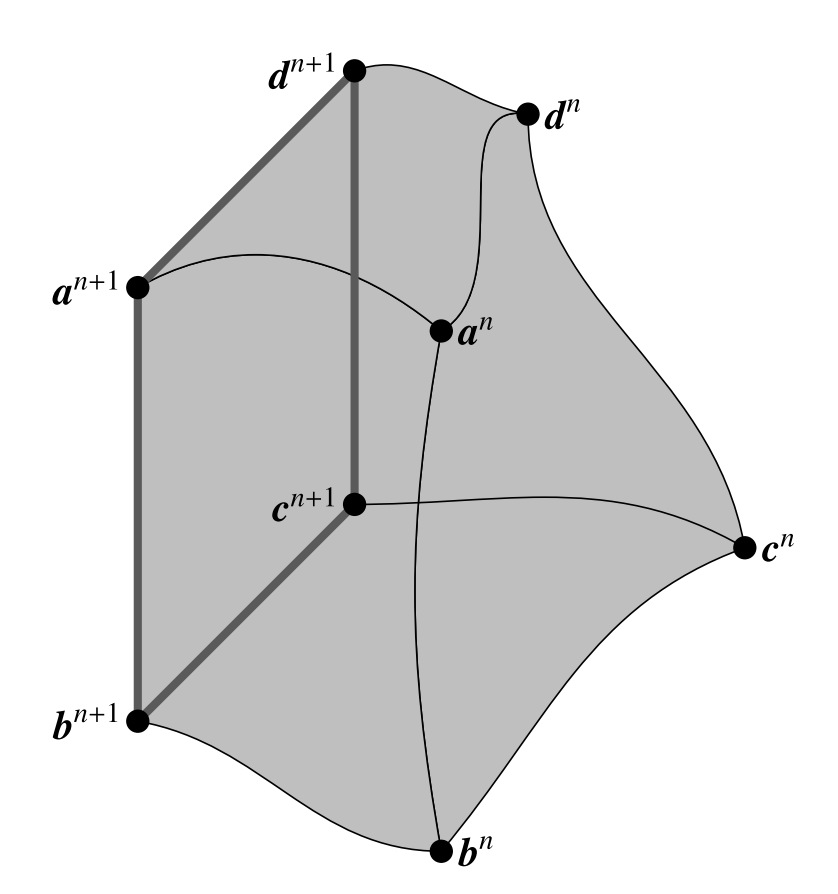
\includegraphics[width=1.0\linewidth]{figs/streaktube.png}
		\caption{The scalar quantity to be advected is approximated and projected out of the control volume for integration over time~\cite{Owkes2014}. }
		\label{fig:streak}
	\end{subfigure}%
\hfill
	\begin{subfigure}{0.45\textwidth}
		\centering
		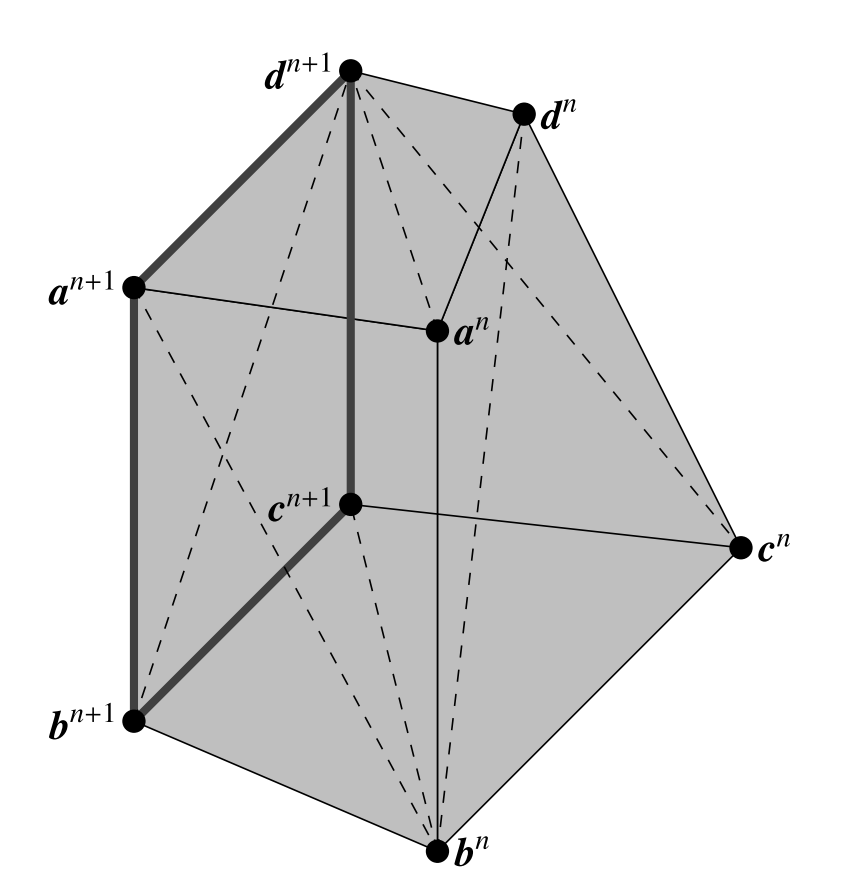
\includegraphics[width=1.0\linewidth]{figs/simplicies}
		\caption{The representative volume is partitioned into simplicies (tetrahedra in 3D) until they are sufficiently small such that the simplicies contain only one phase of fluid~\cite{Owkes2014}.}
		\label{fig:simp}
	\end{subfigure}
\caption{Figures included with permission from Elsevier.}
\end{figure}

\section{Streaktube Derivation}
Assume we have a conserved scalar $f(\bm{x},t)$ that evolves in a solenoidal velocity field as 
\begin{equation}
\frac{\partial f}{\partial t} + \nabla \cdot (\bm{u} f) = 0
\label{eqn:der1}
\end{equation}
where \bm{x} is the spatial coordinate value, $t$ is time, and \bm{u} is the velocity field which is known~\cite{Owkes2014}. Integrating this equation over a time step ($t^n \rightarrow t^{n+1}$) and the area of the control volume while using Gauss' theorem on the advection term, we find 
\begin{equation}
\int_{CV} (  f(\bm{x}, t^{n+1})  - f(\bm{x}, t^{n})  ) dV  + \int_{t^n}^{t^{n+1}} \oint_{CS} f \bm{u} \cdot \bm{n}_{CS} dS dt = 0.
\label{eqn:der2}
\end{equation}
The right term is the surface flux through the control volume and is dependent on $f( \bm{x}, t)$ for $t^n \leq t \leq t^{n+1}$, which is not normally a known quantity. However, a discrete representation of $f( \bm{x}, t^{n})$ is typically known and and update equation can be used to determine $f( \bm{x}, t^{n+1})$. So, the flux is reformulated so that it is solely dependent on $f( \bm{x}, t^{n})$. This is achieved by subdividing the surface of the control volume $CS$ into sub-surfaces $\partial{CS_i}$. On each sub-surface $\partial CS_i$ we can link the flux volume $\Omega_i(t)$ to the bounding surface $\omega_i(t)$. $\Omega_i(t)$ is just the signed volume which flows through the sub-surface $\partial CS_i$ over a given time step $\Delta t$.  The sign of the volume is dependent on the orientation into or out of the control volume and is positive if flowing out of, and negative if flowing into, the control volume~\cite{Owkes2017}. 

Integrating Equation~\ref{eqn:der1} over the flux volume $\Omega_i$ and again using Gauss' theorem on the second term we find 
\begin{equation}
\int_{\Omega_i(t)} \frac{\partial f}{\partial t} dV  + \oint_{\omega_i(t)} f \bm{u} \cdot \bm{n}_{\Omega_i} dS = 0.
\label{eqn:der4}
\end{equation}
Here, $\bm{n}_{\Omega_i}$ is the outward facing normal to the flux volume $\Omega_i(t)$. The bounding surface $\omega_i$ is partitioned as $\omega_{i,F} = \omega_i \cap \partial CS_i = \partial CS_i$, which is fixed and $\omega_{i,M} = \omega_i \backslash \partial CS_i $ which is a material surface~\cite{Owkes2017}. This is valid by defining part of $\omega_i$ as having zero flux of $f$ and therefore must move with the flow. The other portion of $\omega_i$ is defined such that it coincides with $\partial CS_i$, which is fixed in time. Integrating Eq.~\ref{eqn:der4} over time and using the previous partition we find that 
\begin{equation}
\int_{t^n}^{t^{n+1}} \int_{\Omega_i(t)} \frac{\partial f}{\partial t} dV dt + \int_{t^n}^{t^{n+1}} \int_{\omega_{i,M}(t)} f \bm{u} \cdot \bm{n}_{\Omega_i} dS dt + 	\int_{t^n}^{t^{n+1}} \int_{\partial CS_i} f \bm{u} \cdot \bm{n}_{\Omega_i} dS dt = 0.
\label{eqn:der5}
\end{equation}
Because of its similarity to the flux term in Eq.~\ref{eqn:der2}, the right term of the above equation will provide a bridge between the two equations. The remaining terms can be made more clear using Leibniz's method which states 
\begin{equation}
\frac{d}{dt} \int_{\Omega_i(t)} f dV = \int_{\Omega_i(t)} \frac{\partial f}{\partial t} dV + \int_{\omega_{i,M}(t)} f \bm{u} \cdot \bm{n}_{\Omega_i} dS.
\label{eqn:der6}
\end{equation}
With this, we can see that a $\Omega_i(t)$ is a streaktube projected backward in time from the surface $\partial CS_i$ over the time step $\Delta t$. Integrating Eq.~\ref{eqn:der6} with time results in 
\begin{multline}
\int_{\Omega_i(t^{n+1})} f (\bm{x} , t^{n+1}) dV - \int_{\Omega_i(t^{n})} f (\bm{x} , t^{n}) dV  = \\ \int_{t^n}^{t^{n+1}}\int_{\Omega_i(t)} \frac{\partial f}{\partial t} dV dt+ \int_{t^n}^{t^{n+1}} \int_{\omega_{i,M}(t)} f \bm{u} \cdot \bm{n}_{\Omega_i} dS dt.
\label{eqn:der7}
\end{multline}
By definition, $\Omega_i(t^{n+1})$ is zero, making the first term equal to zero. We can adopt the notation that $\Omega_i=\Omega_i(t^{n})$ and call this term the flux volume. Subtracting Eq.~\ref{eqn:der7} from Eq.~\ref{eqn:der5} we find that 
\begin{equation}
\int_{t^n}^{t^{n+1}}\int_{\partial CS_i}  f \bm{u} \cdot \bm{n}_{\Omega_i} dS dt = \int_{\Omega_i} f (\bm{x} , t^{n}) dV, 
\label{eqn:der8}
\end{equation}
which gives us a simple relation between the flux through the sub-surface $\partial CS_i$ and the volume integral over $\Omega_i$.

To obtain a useful time advancement equation we would like to combine Eqn.~\ref{eqn:der2} and Eqn.~\ref{eqn:der8}. However, doing so requires a relation between the normal terms, $\bm{n}_{CV}$ and $\bm{n}_{\Omega}$ as these normals are both defined using the same surface. This means that either, the two normals are identical or face opposite directions. We adopt a signed volume convention where the volume is positive if $\bm{n}_{CV} = \bm{n}_{\Omega}$ and negative otherwise. This convention results in positive volumetric fluxes out of the control volume and negative fluxes into the control volume. With this relationship we can finally obtain 
\begin{equation}
\int_{CV} (f (\bm{x} , t^{n+1}) - f (\bm{x} , t^{n}) )dV + \sum_{i=1}^{N_S}\int_{\Omega_S} f (\bm{x} , t^{n}) )dV =0
\label{eqn:derFinal}
\end{equation}
where $\Omega_S$ is now the signed streaktube. The final form provides that the change in the scalar $f$  within the control volume $CV$ over the timestep $\Delta t$ must be equal to the volume integral of the signed flux volumes. 
%\begin{figure}
%	\centering
%	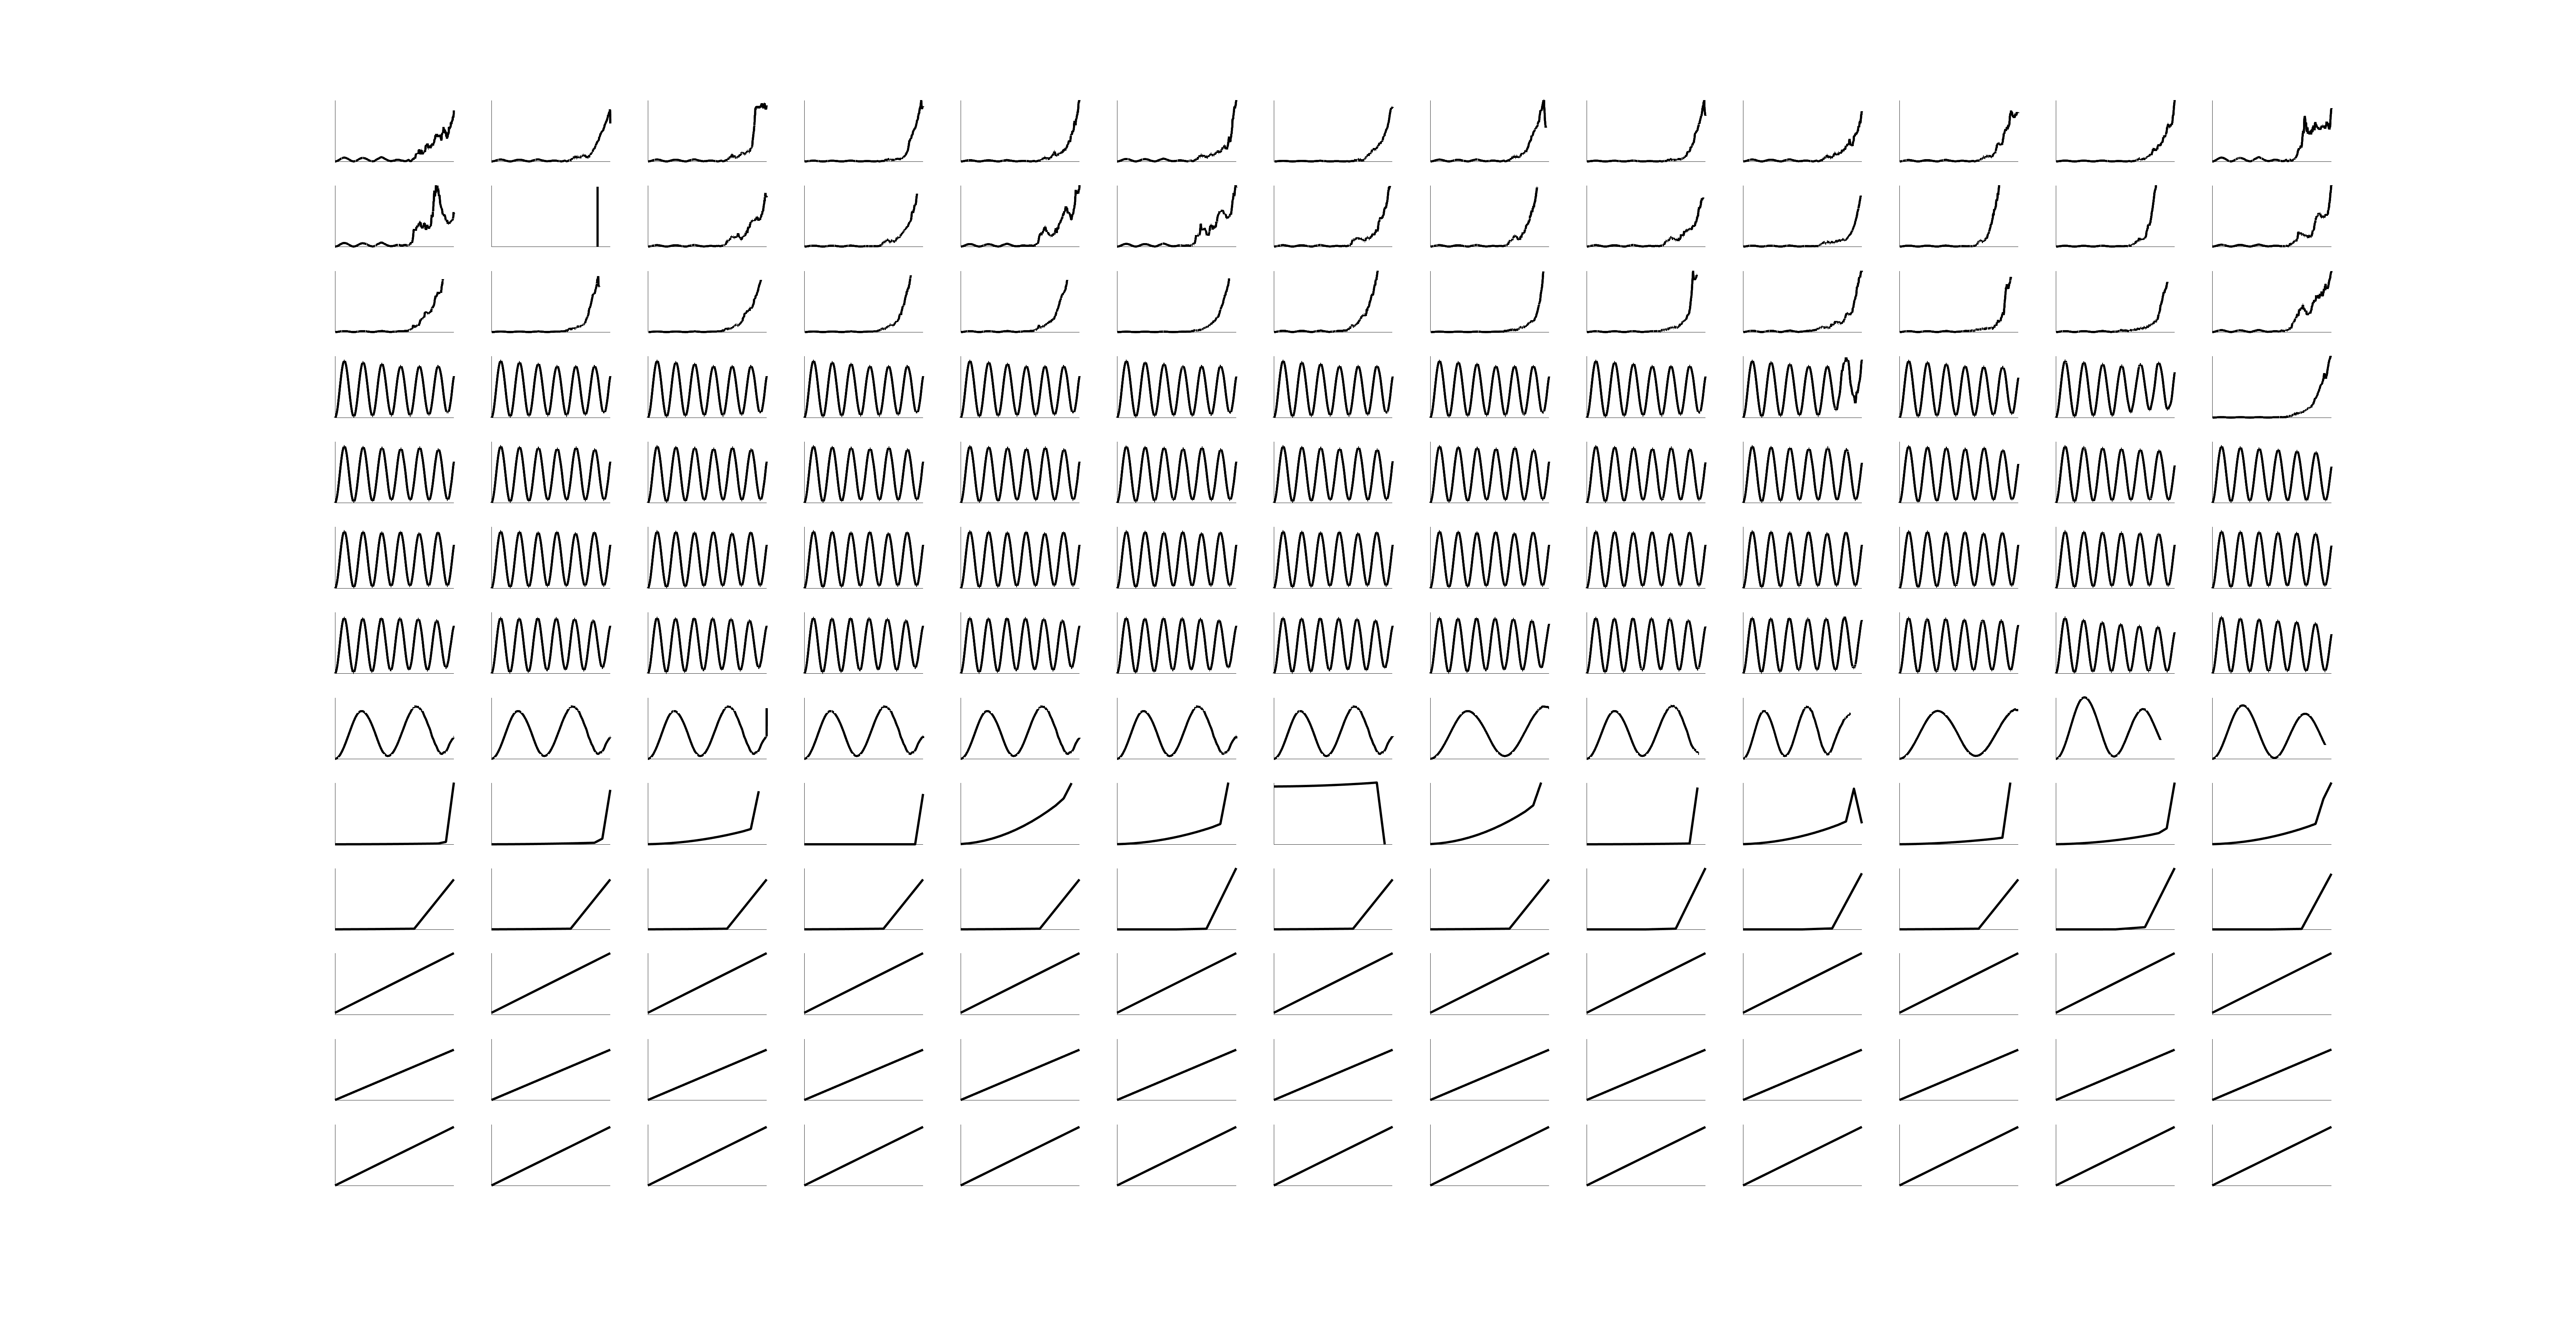
\includegraphics[width=1.0\textwidth]{figs/para}
%	\caption{fix figure}
%	\label{fig:para}
%\end{figure}

\section{Mesh Generation}
In numerical analysis, the grid or mesh, often refers to the manner in which a domain being simulated is subdivided into smaller sections and points. The type of grid used can be classified as being in one of two categories, structured or unstructured~\cite{anderson}. The choice of whether to use a structured or unstructured grid should be considered on a case by case basis. However, there are some defining characteristics of each that are important to recognize prior to implementation. A structured grid in 2D can be thought of a series of quadrilateral elements (bricks) placed side by side in a uniform fashion~\cite{MIT}. Here, neighboring elements are referenced by adding or subtracting from the base cell indices as indicated below~\cite{anderson}. Figure~\ref{fig:ijGrid} is an example of a structured grid. An unstructured grid, as in Figure~\ref{fig:Unstructured Grid}, does not retain uniformity and is often comprised of triangular, rectangular, or hexagonal elements in 2D applications~\cite{tu}. To reference neighboring cells in an unstructured grid, storage of cell-to-cell pointers are required~\cite{MIT}. Unstructured grids normally require a greater amount of memory storage and can result in slower computation times than that of a structured grid~\cite{magoules}. A simplified example of an unstructured grid can be referenced in Figure~\ref{fig:Unstructured Grid}. The NGA code, which is this focus of this research, uses a structured grid approach for simplicity and computational efficiency. However, it should be noted that unstructured grids are increasing in popularity as the accuracy obtained from modeling complex flow geometry may be higher than that of a structured grid~\cite{Hirt1981}. 

\begin{figure}[htbp]
	\centering
	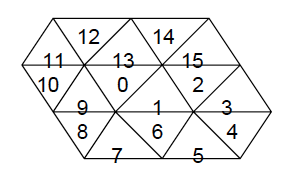
\includegraphics[width=0.5\textwidth]{figs/unstruc}
	\caption{Simple Unstructured Grid \cite{MIT}}
	\label{fig:Unstructured Grid}
\end{figure}

For a Cartesian mesh, these points are organized using an $i$ and $j$, with $i$ providing the $x$ location and $j$ the $y$ location as seen in Figure \ref{fig:ijGrid}. For example, if a value is being calculated at the $(i,j)$ cell and requires information from the neighbors to the left and right, the neighbors are referenced as $(i-1,j)$ and $(i+1,j)$ respectively. If the calculation requires information from neighbors on the top and bottom however, the cells are referenced as $(i,j+1)$ and $(i,j-1)$. This method is extended similarly in the z-direction for 3D applications~\cite{MIT}. 
\begin{figure}[htbp]
	\centering
	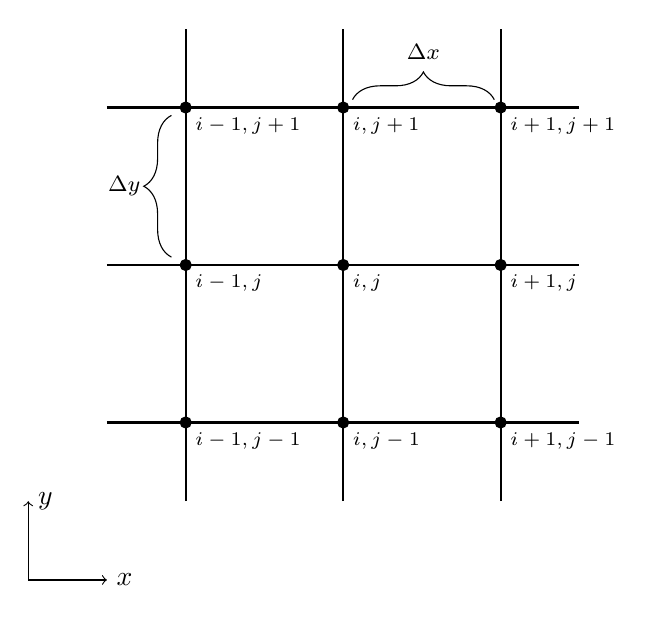
\begin{tikzpicture}[scale=2.0]
	% Mesh
	\draw [black,thick,step=1.0] (0.5 , 0.5) grid (3.5,3.5); 
	% i's and j's
	\node[below right] at (1,1) {\scriptsize{$i-1,j-1$}};
	\node[below right] at (1,2) {\scriptsize{$i-1,j$}};
	\node[below right] at (1,3) {\scriptsize{$i-1,j+1$}};
	\node[below right] at (2,1) {\scriptsize{$i,j-1$}};
	\node[below right] at (2,2) {\scriptsize{$i,j$}};
	\node[below right] at (2,3) {\scriptsize{$i,j+1$}};
	\node[below right] at (3,1) {\scriptsize{$i+1,j-1$}};
	\node[below right] at (3,2) {\scriptsize{$i+1,j$}};
	\node[below right] at (3,3) {\scriptsize{$i+1,j+1$}};
	%Node Circles
	\foreach \x in {1,...,3} {
		\foreach \y in {1,...,3} {
			\draw [fill] (\x,\y) circle [radius=0.035];
		}
	}                  
	%Axes
	\draw [arrows=->] (0,0) -- node[pos=1,right] {$\bm{x}$} (0.5,0);
	\draw [arrows=->] (0,0) -- node[pos=1,right] {$\bm{y}$} (0,0.5);
	%Dx Dy
	\draw [decorate,decoration={brace,amplitude=10pt},xshift=-4pt,yshift=0pt] (1.05,2.05) -- (1.05,2.95) node [black,midway,xshift=-0.6cm] {\footnotesize $\Delta y$};
	\draw [decorate,decoration={brace,amplitude=10pt},xshift=-4pt,yshift=0pt] (2.2,3.05) -- (3.1,3.05) node [black,midway,yshift=0.6cm] {\footnotesize $\Delta x$};
	\end{tikzpicture}
	\caption{Typical $(i,j)$ notation of structured grid cells. Grid cells span $\Delta x$ and $\Delta y$ in the horizontal and vertical directions respectively. }
	\label{fig:ijGrid}
\end{figure}


\section{Rudman Dual Grid Formulation}
Solution of the incompressible Navier-Stokes equations traditionally occurs on whats known as a staggered grid. On a staggered grid, pressure is typically stored at cell centers and velocity components are stored at cell faces~\cite{TRYG}. Building from the structured grid example given in Figure~\ref{fig:ijGrid}, the staggered grid is illustrated in Figure~\ref{fig:StagGrid}. 
\begin{figure}[htbp]
	\centering
	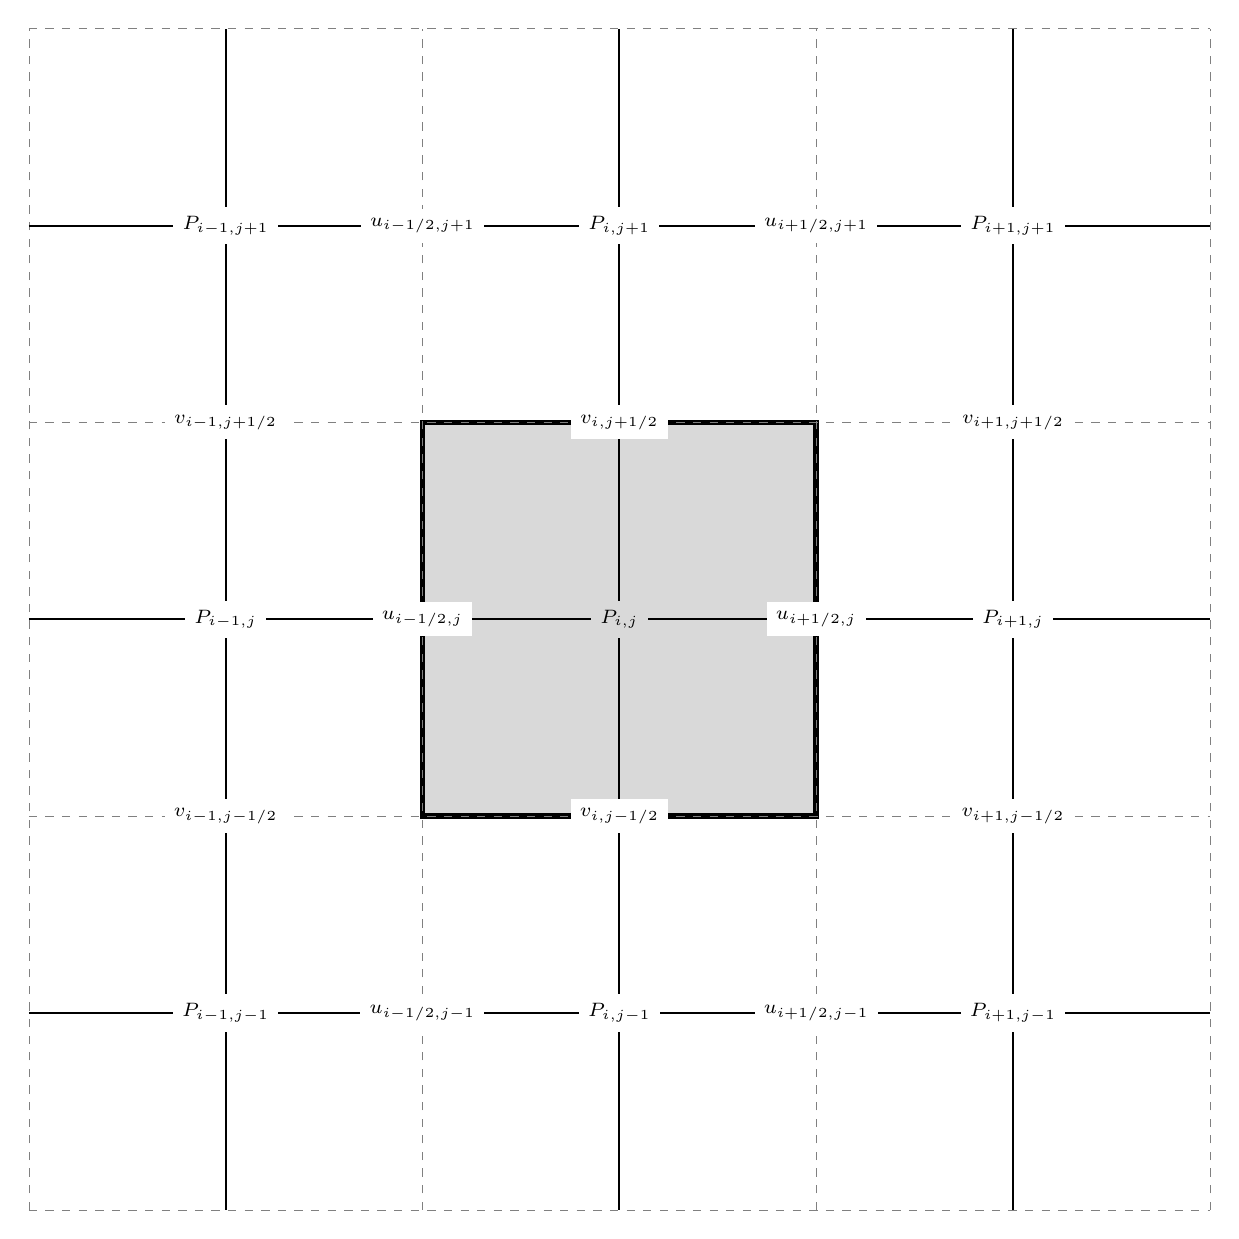
\begin{tikzpicture}[scale=5.0]
	% Mesh
	\draw [black, fill=gray!30] (1.5,1.5) rectangle (2.5,2.5);
	\draw [black, line width = 2pt] (1.5,1.5) rectangle (2.5,2.5);
	\draw [dashed, step=0.5, help lines] (0.5,0.5) grid (3.5,3.5);
	\draw [black,thick,step=1.0] (0.5 , 0.5) grid (3.5,3.5); 
	% i's and j's
	\node[fill=white]    at (1,1) {\scriptsize{$P_{i-1,j-1}$}};
	\node[fill=white]    at (1,2) {\scriptsize{$P_{i-1,j}$}};
	\node[fill=white]    at (1,3) {\scriptsize{$P_{i-1,j+1}$}};
	\node[fill=white]    at (2,1) {\scriptsize{$P_{i,j-1}$}};
	\node[fill=gray!30] at (2,2)  {\scriptsize{$P_{i,j}$}};
	\node[fill=white]    at (2,3) {\scriptsize{$P_{i,j+1}$}};
	\node[fill=white]    at (3,1) {\scriptsize{$P_{i+1,j-1}$}};
	\node[fill=white]    at (3,2) {\scriptsize{$P_{i+1,j}$}};
	\node[fill=white]    at (3,3) {\scriptsize{$P_{i+1,j+1}$}};
	
	\node[fill=white]    at (1.5,1) {\scriptsize{$u_{i-1/2,j-1}$}};
	\node[fill=white]    at (1.5,2) {\scriptsize{$u_{i-1/2,j}$}};
	\node[fill=white]    at (1.5,3) {\scriptsize{$u_{i-1/2,j+1}$}};
	
	\node[fill=white]    at (2.5,1) {\scriptsize{$u_{i+1/2,j-1}$}};
	\node[fill=white]    at (2.5,2) {\scriptsize{$u_{i+1/2,j}$}};
	\node[fill=white]    at (2.5,3) {\scriptsize{$u_{i+1/2,j+1}$}};
	
	\node[fill=white]    at (1,1.5) {\scriptsize{$v_{i-1,j-1/2}$}};
	\node[fill=white]    at (1,2.5) {\scriptsize{$v_{i-1,j+1/2}$}};

	
	\node[fill=white]    at (2,1.5) {\scriptsize{$v_{i,j-1/2}$}};
	\node[fill=white]    at (2,2.5) {\scriptsize{$v_{i,j+1/2}$}};

	\node[fill=white]    at (3,1.5) {\scriptsize{$v_{i+1,j-1/2}$}};
	\node[fill=white]    at (3,2.5) {\scriptsize{$v_{i+1,j+1/2}$}};
	
	\end{tikzpicture}
	\caption{Typical notation of structured grid cells. For each cell, pressure values are stored at the center of the control volume, shaded in gray here. Velocity components are stored at the center of the cell faces. }
	\label{fig:StagGrid}
\end{figure}
This approach was first introduced by Harlow and Welch (1965) and is now considered the standard approach in structured mesh CFD applications~\cite{HARLOW1965}. For incompressible flows, staggered grids offer the advantage of tightly coupling fluid property variables as well as eliminating pressure-velocity checkerboarding~\cite{rudman}. The Rudman dual grid approach, first presented by Rudman (1998), is a technique developed for high density ratio, multiphase flows, which accurately conserves both mass and momentum. This is achieved by calculating density-fluxes on a twice as fine mesh near the fluid interface as illustrated in Figure~\ref{fig:StagGrid}~\cite{rudman}. Without  this method implemented, density is stored at cell faces while density-flux is calculated at cell centers. This can allow for a problematic disconnect between the calculated density and flux values. The Rudman dual mesh is incorporated into NGA and is essential to the formulation of the method presented in this research.


\section{Interface Tracking Schemes}%\todo{Should have a broader section on interface tracking and capturing schemes and explain why VOF is often used.}\todo{give mathematical definition of volume of fluid} 
In order to accurately predict the behavior of a multiphase system, the location of the interface of the two fluids must be determined. Popular methods for achieving this interface tracking include the Front Tracking method, the Level-set method, and Phase-field methods\cite{TRYG}. The Front Tracking method of Unverdi and Tryggvason (1992) tracks the interface with a number of marker points on the interface which are advected with the velocity field and interpolated from the fixed mesh~\cite{UNVERDI}. The Level-set method identifies the different fluids with a marker function whereby one fluid is identified as positive and the other, negative~\cite{OSHER}. The interface exists at the zero level-set. Phase-field methods assume the interface has a finite thickness and uses thermodynamic conservation laws to describe it~\cite{JACQMIN}. Further information about each of these methods can be found in~\cite{TRYG}.

\section{Volume of Fluid Formulation}
One additional method for completing this interface tracking is known as the Volume of Fluid (VOF) method. This method was first introduced by Hirt \& Nichols (1981) and has been expanded upon since its original implementation~\cite{Hirt1981,TRYG}. The defining contribution of the VOF method proposed by Hirt~\&~Nichols is the introduction of a scalar marker function assigned to each mesh cell which is indicative of the volume of a given fluid within that cell~\cite{Hirt1981}. This allows for interface to be tracked by the value of the marker cell in surrounding cells. For example, if $VOF = 1.0$ indicates a region of liquid and $VOF = 0.0$ indicates a region of gas, then a cell with a value $0.0 \leq VOF \leq 1.0$ indicates a cell which contains interface. A one-dimensional example of this advection can be seen in Figure \ref{fig:1Dadvect}. It is important to recognize that for 1D flow, volume of a fluid may only be advected into a new cell once the current cell is full~\cite{TRYG}. However, this is not true for cases of increased dimensionality and advection criteria can become tedious for 2D and 3D flow fields. 
\begin{figure}[htbp]
	\begin{subfigure}[b]{1.0\textwidth}
		\centering
	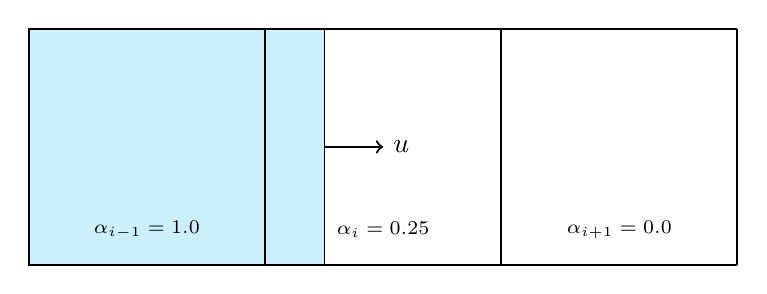
\begin{tikzpicture}[scale=3.0]
	% Mesh
	\draw [black,fill=cyan!20] (0.0,0.0) -- (1.25,0.0) -- (1.25,1.0) -- (0.0,1.0) -- cycle;
	\draw [black,thick,step=1.0] (0.0 , 0.0) grid (3.0,1.0); 
	%Velocity
	\draw [arrows=->, thick] (1.25,0.5) -- node[pos=1,right] {$u$} (1.5,0.5);
	%Labels
	\node[] at (0.5,0.15) {\scriptsize{$\alpha_{i-1}=1.0$}};
	\node[] at (1.5,0.15) {\scriptsize{$\alpha_{i}=0.25$}};
	\node[] at (2.5,0.15) {\scriptsize{$\alpha_{i+1}=0.0$}};
	\end{tikzpicture}
	\caption{A fluid interface exists within a velocity field. Cells volume fractions ($\alpha$) are calculated. }
	\label{fig:1Dadvect1}
	\end{subfigure}

	\begin{subfigure}[b]{1.0\textwidth}
		\centering
	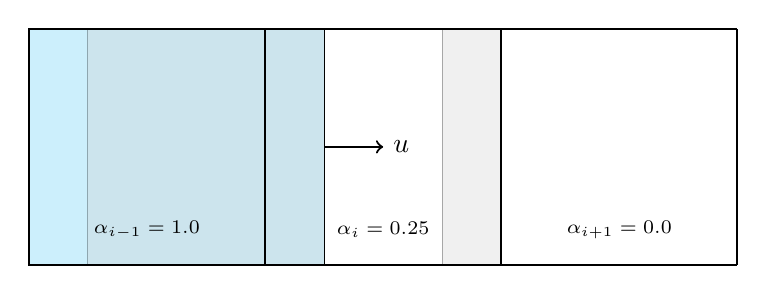
\begin{tikzpicture}[scale=3.0]
	% Mesh
	\draw [black,fill=cyan!20] (0.0,0.0) -- (1.25,0.0) -- (1.25,1.0) -- (0.0,1.0) -- cycle;
	\draw [black,fill=gray!40, opacity=0.3] (0.25,0.0) -- (1.25,0.0) -- (1.25,1.0) -- (0.25,1.0) -- cycle;
	\draw [black,fill=gray!40, opacity=0.3] (1.75,0.0) -- (2.0,0.0) -- (2.0,1.0) -- (1.75,1.0) -- cycle;
	\draw [black,thick,step=1.0] (0.0 , 0.0) grid (3.0,1.0); 
	%Velocity
	\draw [arrows=->, thick] (1.25,0.5) -- node[pos=1,right] {$u$} (1.5,0.5);
	%Labels
	%Labels
	\node[] at (0.5,0.15) {\scriptsize{$\alpha_{i-1}=1.0$}};
	\node[] at (1.5,0.15) {\scriptsize{$\alpha_{i}=0.25$}};
	\node[] at (2.5,0.15) {\scriptsize{$\alpha_{i+1}=0.0$}};
	\end{tikzpicture}
	\caption{The amount of fluid to be fluxed through a face is determined using streak tubes.}
	\label{fig:1Dadvect2}
	\end{subfigure}

	\begin{subfigure}[b]{1.0\textwidth}
		\centering
	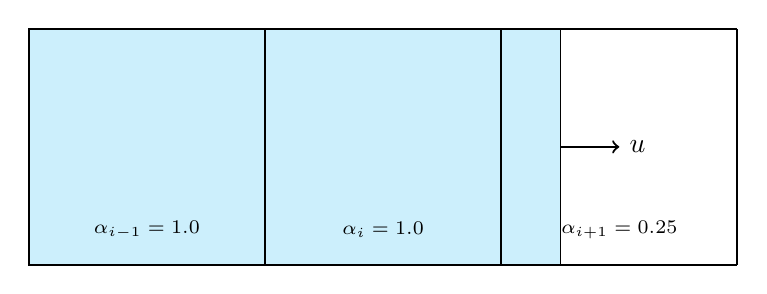
\begin{tikzpicture}[scale=3.0]
	% Mesh
	\draw [black,fill=cyan!20] (0.0,0.0) -- (2.25,0.0) -- (2.25,1.0) -- (0.0,1.0) -- cycle;
%	\draw [black,fill=gray!40, opacity=0.3] (1.25,0.0) -- (2.25,0.0) -- (2.25,1.0) -- (1.25,1.0) -- cycle;
	\draw [black,thick,step=1.0] (0.0 , 0.0) grid (3.0,1.0); 
	%Velocity
	\draw [arrows=->, thick] (2.25,0.5) -- node[pos=1,right] {$u$} (2.5,0.5);
	%Labels
	%Labels
	\node[] at (0.5,0.15) {\scriptsize{$\alpha_{i-1}=1.0$}};
	\node[] at (1.5,0.15) {\scriptsize{$\alpha_{i}=1.0$}};
	\node[] at (2.5,0.15) {\scriptsize{$\alpha_{i+1}=0.25$}};
	\end{tikzpicture}
	\caption{The fluid is advanced through the cell.}
	\label{fig:1Dadvect3}
	\end{subfigure}
	\caption{Advection of a one-dimensional fluid interface}
\label{fig:1Dadvect}
\end{figure}

The advection procedure for a VOF method is completed in two primary steps. First, the interface needs to be geometrically constructed. Second, the constructed interface is advected with the current velocity field~\cite{TRYG}. Figure~\ref{fig:1Dadvect} depicts one-dimensional interface advection. In this case, geometric reconstruction is accomplished with a single vertical line. Adoption of this method is straightforward. As simulations increase to two or three dimensional analysis however, this problem quickly becomes non-trivial. Early attempts to resolve this difficulty include the Simple Line Interface Calculation (SLIC) method of Noh and Woodward (1976)~\cite{nohwoodward}. Here, the reconstructed interface is made up of lines which align parallel to the mesh in both \textit{x} and \textit{y} directions as in Figure~\ref{fig:SLIC} where the true interface is depicted in Figure~\ref{fig:trueSlic}.           
\begin{figure}[htbp]
	\begin{subfigure}[b]{0.45\linewidth}
	\centering
%	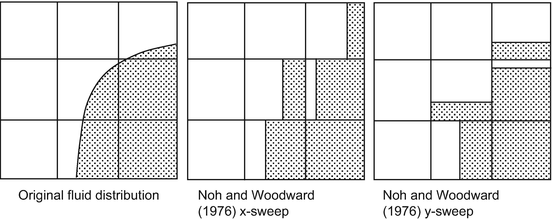
\includegraphics[width=1.0\textwidth]{figs/SLIC.png}
	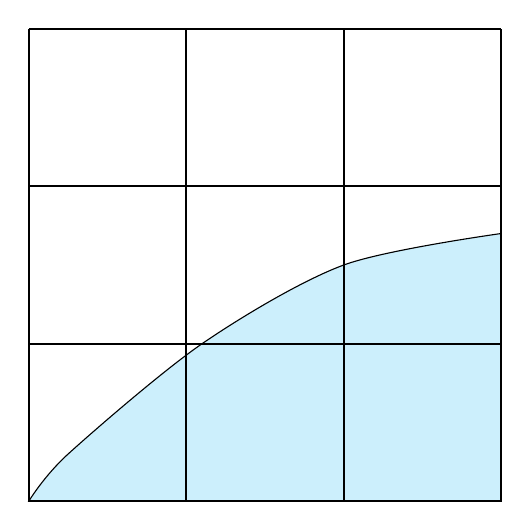
\begin{tikzpicture}[scale=2.0]
	% Mesh
	\draw [black, fill=cyan!20] plot [smooth ] coordinates {(0,0)(0.25,0.3)(1.1,1)(2,1.5)(3,1.7)} -- (3,0) -- cycle;
	\draw [black,thick,step=1.0] (0.0,0.0) grid (3.0,3.0);
	\end{tikzpicture}
	\caption{True Interface}
	\label{fig:trueSlic}
	\end{subfigure}
\hfill
	\begin{subfigure}[b]{0.45\linewidth}
	\centering
	%	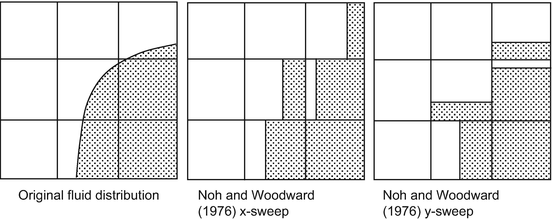
\includegraphics[width=1.0\textwidth]{figs/SLIC.png}
	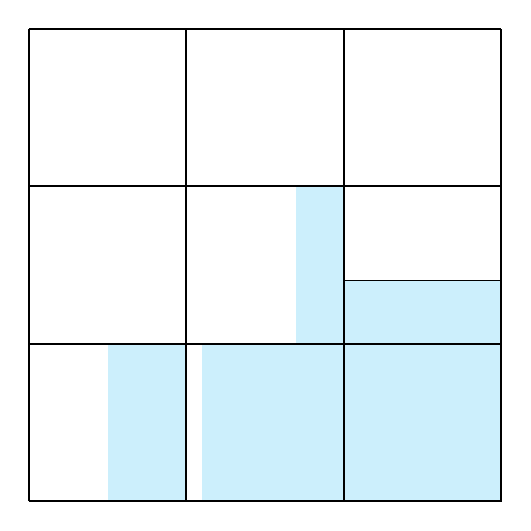
\begin{tikzpicture}[scale=2.0]
	% Mesh
	\draw [black, fill=cyan!20] (0.5,0)-- (1,0) -- (1,1) -- (0.5,1);
	\draw [black, fill=cyan!20] (1.1,0)-- (3,0) -- (3,1) -- (1.1,1);
	\draw [black, fill=cyan!20] (2,1)-- (3,1) -- (3,1.4) -- (2,1.4);
	\draw [black, fill=cyan!20] (1.7,1)-- (2,1) -- (2,2) -- (1.7,2);
	\draw [black,thick,step=1.0] (0.0,0.0) grid (3.0,3.0);
	\end{tikzpicture}
	\caption{SLIC Approximation}
	\label{fig:SLIC}
	\end{subfigure}
	\caption{SLIC method of Noh and Woodward (1976)}
\end{figure}
Improvement to the SLIC method was presented by Youngs (1982)  known as the Piecewise Linear Interface Calculation (PLIC)~\cite{youngs}. In the PLIC method, instead of aligning interfacial reconstruction lines with the mesh, a line (2D) or plane (3D) is oriented with a normal vector which is evaluated from the volume fraction gradient~\cite{tu}. An example of PLIC can be seen in Figure~\ref{fig:PLIC} where the true interface is represented in Figure~\ref{fig:truePlic}. This method is a popular geometric reconstruction scheme still today and is used in NGA for this research.

\begin{figure}[htbp]
	\begin{subfigure}[b]{0.45\linewidth}
		\centering
		%	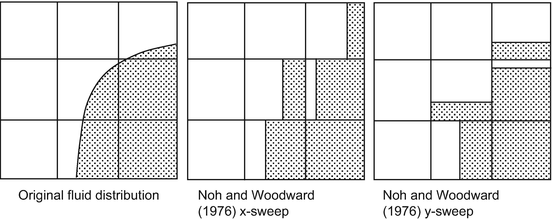
\includegraphics[width=1.0\textwidth]{figs/SLIC.png}
		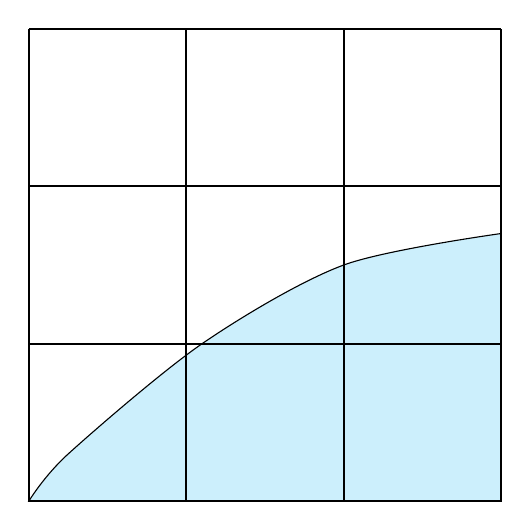
\begin{tikzpicture}[scale=2.0]
		% Mesh
		\draw [black, fill=cyan!20] plot [smooth ] coordinates {(0,0)(0.25,0.3)(1.1,1)(2,1.5)(3,1.7)} -- (3,0) -- cycle;
		\draw [black,thick,step=1.0] (0.0,0.0) grid (3.0,3.0);
		\end{tikzpicture}
		\caption{True Interface}
		\label{fig:truePlic}
	\end{subfigure}
	\hfill
	\begin{subfigure}[b]{0.45\linewidth}
		\centering
		%	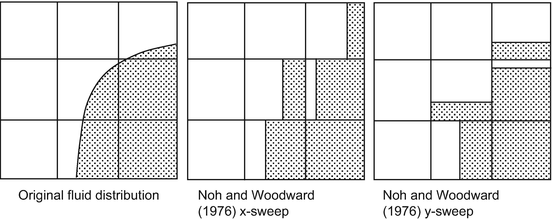
\includegraphics[width=1.0\textwidth]{figs/SLIC.png}
	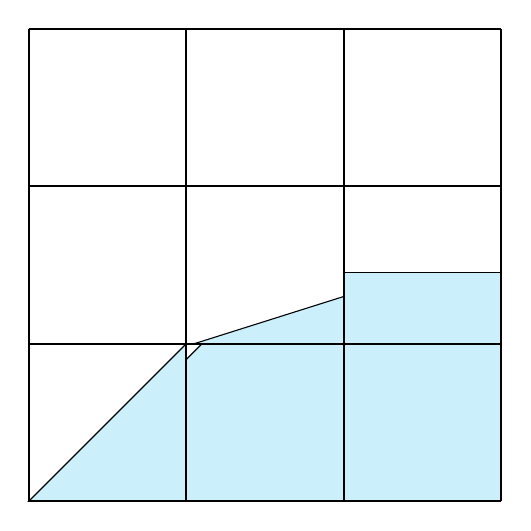
\begin{tikzpicture}[scale=2.0]
	% Mesh
	\draw [black, fill=cyan!20] (0,0)-- (1,0) -- (1,1) -- cycle;
	\draw [black, fill=cyan!20] (1,0)-- (2,0) -- (2,1) -- (1.1,1) --(1,0.9) ;
	\draw [black, fill=cyan!20] (1.05,1)-- (2,1) -- (2,1.3) -- cycle;
	\draw [black, fill=cyan!20] (2,0)-- (2,1.45) -- (3,1.45) -- (3,0);
	\draw [black,thick,step=1.0] (0.0,0.0) grid (3.0,3.0);
	\end{tikzpicture}
		\caption{PLIC Approximation}
		\label{fig:PLIC}
	\end{subfigure}
	\caption{Piecewise Linear Interface Calculation of Youngs (1982) }
\end{figure}

\section{Curvature Estimation - Height Function Methods}
Curvature can be discretely described as the reciprocal of radius of a given surface as illustrated in Figure \ref{fig:curv}~\cite{Owkes2018}. 
 \begin{figure}[htbp]
	\centering
	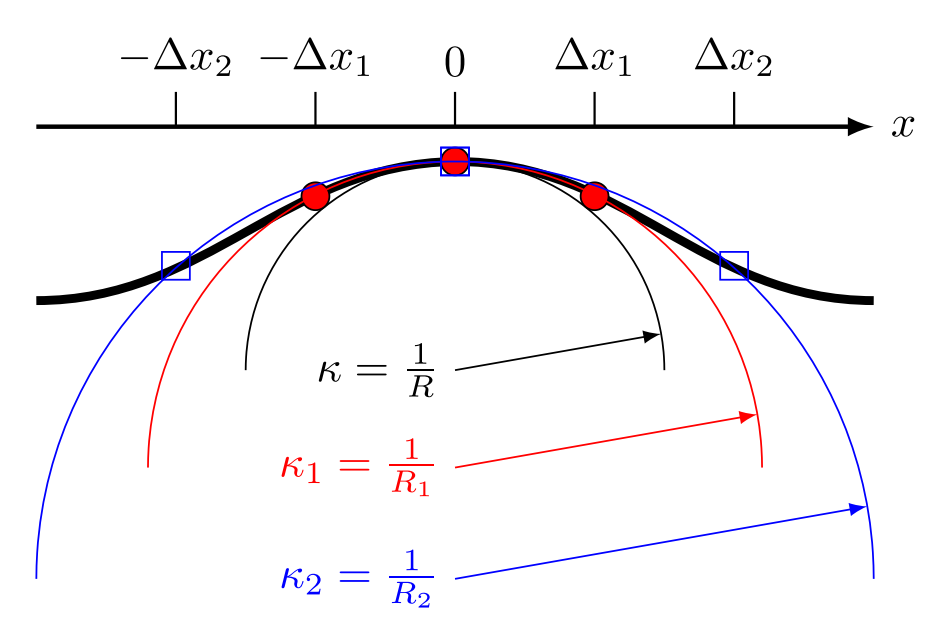
\includegraphics[width=0.5\textwidth]{figs/curv}
	\caption{Curvature calculations for varying radii. Curvature can be calculated as the reciprocal of the radius of a curve~\cite{Owkes2018}.}
	\label{fig:curv}
\end{figure}
Accurate simulations of multiphase flows require an accurate estimation of interface curvature. Figure \ref{fig:surf} illustrates this importance by presenting experimental results of breakup. These simulations vary only by their Weber number,
\begin{equation}
We= \frac{\rho \bm{u}^2 D}{\sigma},
\end{equation}
 which is inversely proportional to the surface tension term, and thereby, the curvature at the interface. It is clear that the structure seen in Figure~\ref{fig:surf}(d) is experiencing far greater breakup than that seen in Figure~\ref{fig:surf}(a). The correct representation of reality is highly dependent on the estimation of curvature made by the numerical model. 
 \begin{figure}[htbp]
	\centering
	\includegraphics[width=0.5\textwidth]{figs/breakup.png}
	\caption{Atomization simulations with varying Weber number, (a)$We=20$, (b)$We=40$, (c)$We=80$, (d)$We=120$. Adopted with permission from Royal Society Publishing.}
	\label{fig:surf}
\end{figure}

The focus of this work is on modified height function methods which are one method of curvature evaluation.
 \begin{figure}[htbp]
	\centering
	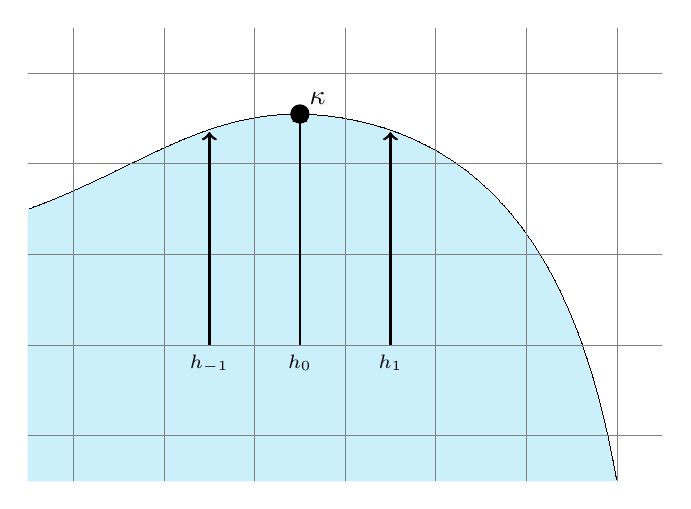
\begin{tikzpicture}[scale=1.15]
		% Mesh
		\draw [step=1.0, help lines] (0.5,0.5) grid (7.5,5.5);
		% Liquid
		\draw [line width=0,fill=cyan!20] (0.5,3.5) to[out=20,in=170] (4,4.5) to[out=-10,in=100] (7.0,0.5);
		\draw [cyan!20,fill=cyan!20] (0.5,3.5) -- (7.0,0.5) -- (0.5,0.5) -- cycle;
		\draw [step=1.0, help lines] (0.5,0.5) grid (7.5,5.5);
		% kappa 1
		\draw [fill] (3.5,4.55) circle [radius=0.1];
		\node [above right] at (3.5,4.55) {$\kappa$};
		\draw [arrows=->,line width=1.0] (2.5,2) -- (2.5,4.35);\node [below] at (2.5,2) {\scriptsize $h_{-1}$};
		\draw [arrows=->,line width=1.0] (3.5,2) -- (3.5,4.55);\node [below] at (3.5,2) {\scriptsize $h_{0}$};
		\draw [arrows=->,line width=1.0] (4.5,2) -- (4.5,4.35);\node [below] at (4.5,2) {\scriptsize $h_{1}$};
		% Triad
%		\begin{scope}[shift={(0.5,0.5)}] 
%			\draw [arrows=->] (0,0) -- node[pos=1,right] {$\bm{x}$} (0.5,0);
%			\draw [arrows=->] (0,0) -- node[pos=1,right] {$\bm{y}$} (0,0.5);
%		\end{scope}
	\end{tikzpicture}
	\caption{Traditional height function with a three cell stencil.} 
	\label{fig:hts}
\end{figure}
Height functions work by summing volume fractions ($\alpha$) within columns of cells to form heights as 
\begin{equation}
h_{i} = \sum_{j-N}^{j+N} \alpha_{i,j} \Delta y
\label{eqn:hts}
\end{equation}
where $N$ represents the number of cells above and below the cell of interest to construct the column. Figure~\ref{fig:hts} gives an example of heights at a liquid-gas interface. In the simplest execution of a height function, approximation of the curvature ($\kappa$) at the point on the grid is achieved by using a simple finite difference of the heights to approximate first and second derivatives as 
\begin{equation}
H_{x} = \frac{h_{i-1}-h_{i+1}}{2 \Delta x}
\label{eqn:1st}
\end{equation}
\begin{equation}
H_{xx} = \frac{h_{i+1}-2h_{i}+h_{i-1}}{ \Delta x^2}.
\label{eqn:2nd}
\end{equation}
Finally, curvature is calculated using
\begin{equation}
\kappa = \frac{-H_{xx}}{(1+H_{x}^{2})^{\frac{3}{2}}}.
\label{eqn:kap}
\end{equation}
Clearly the above explanation is relevant for two dimensional flows. Extension to three dimensional flows requires two dimensional approximations of derivatives and results in a curvature calculation of 
\begin{equation}
\kappa = \frac{-H_{xx}-H_{yy}-H_{xx}H_y^2-H_{yy}H_x^2+2H_{xy}H_xH_y}{(1+H_{x}^{2}+H_{y}^{2})^{\frac{3}{2}}}.
\label{eqn:kap3D}
\end{equation}
A similar approach is taken using widths where an interface is more vertical than horizontal. The height function method requires well defined heights; heights which are completely composed of a single fluid (liquid in our examples). Well defined heights require that columns are constructed of only one phase of fluid above and below the cell that curvature is being calculated at. Figure~\ref{fig:probhts} gives a good depiction of ill-defined heights. In this figure, we can see that The green columns only contain liquid below the interface. However, the red columns have to pass from liquid to gas and then back into liquid to build a proper column. These heights can be considered ill-defined. 
\begin{figure}
	\centering
	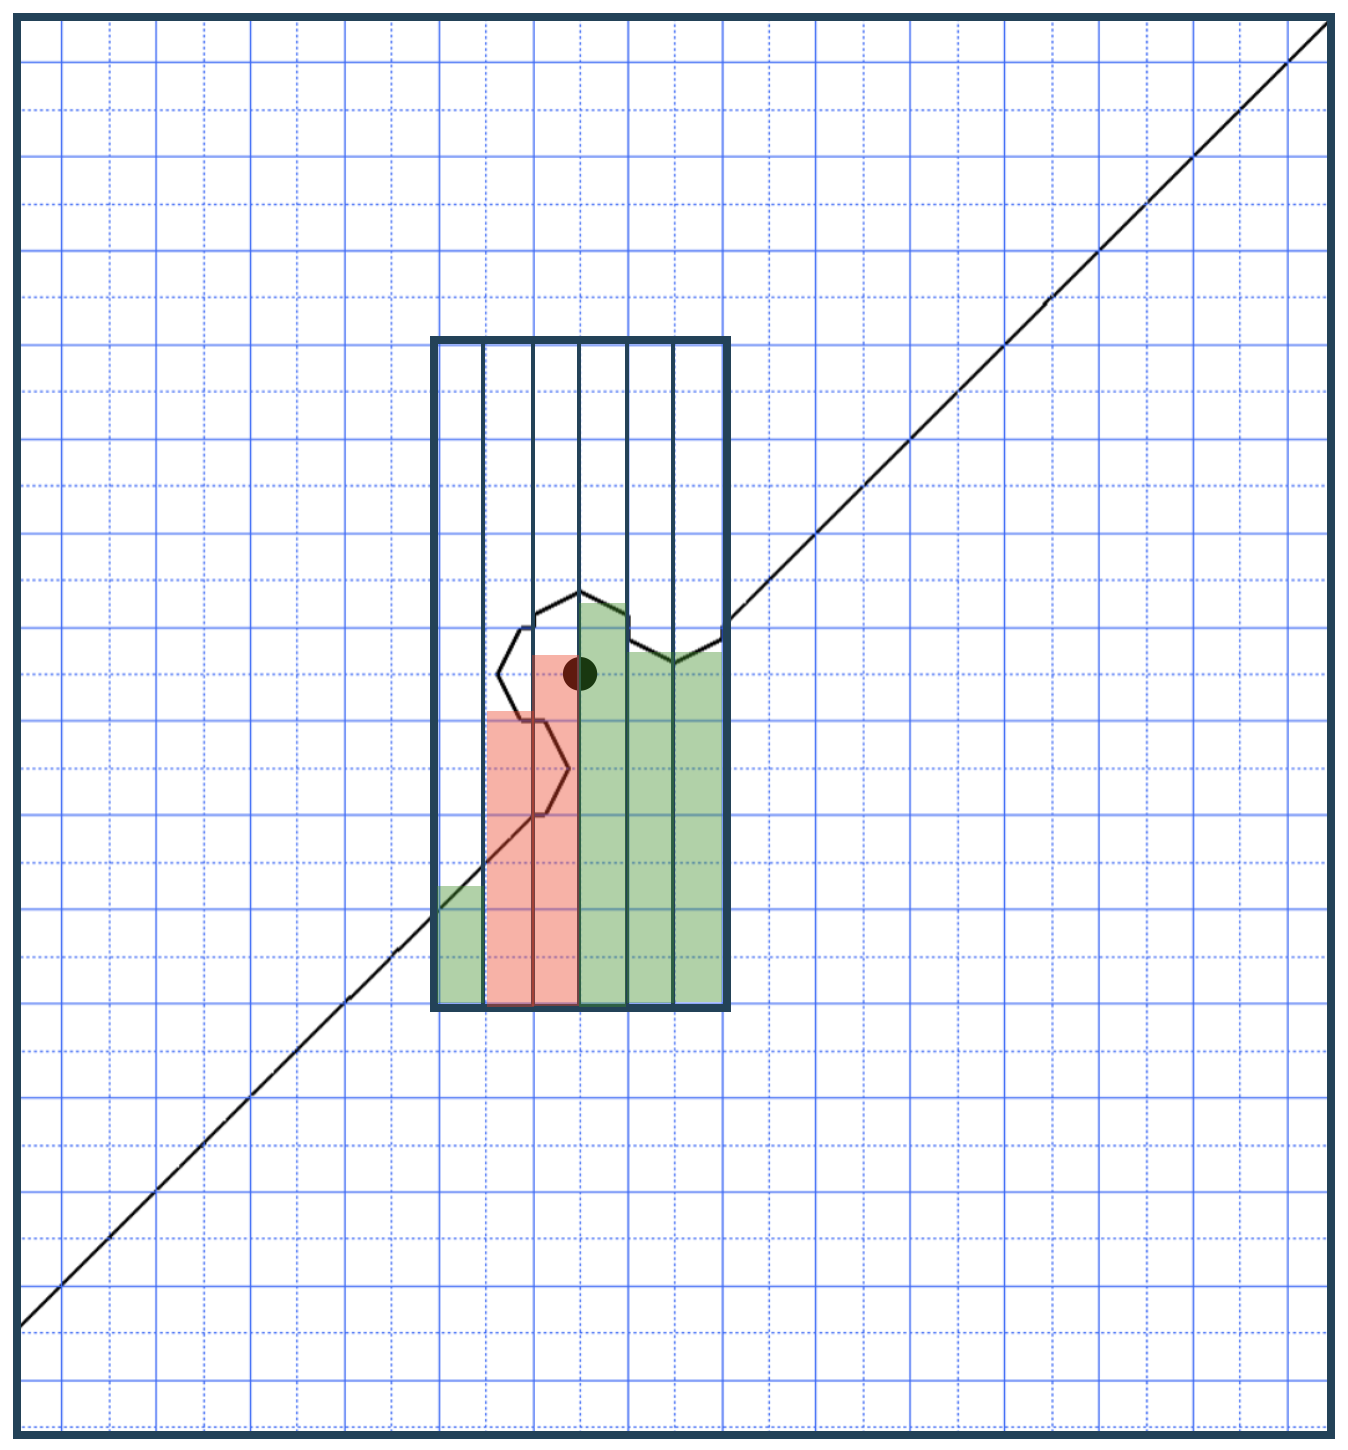
\includegraphics[width=0.5\linewidth]{figs/probhts.png}
	\caption{For the diagonal protrusion test case it is evident that the height function is unable to create the necessary well defined heights that are required for an accurate curvature estimation when a protrusion is on the order of a coarse grid cell.}
	\label{fig:probhts}
\end{figure}
 For interfaces which are mostly vertical, using heights as we've described thus far would not allow for well defined heights. Instead, using the same methodology to build widths allows for properly defined heights with which to calculate curvature. Figure~\ref{fig:widths} provides an example where using heights is the most appropriate choice.
 \begin{figure}[htbp]
	\centering
	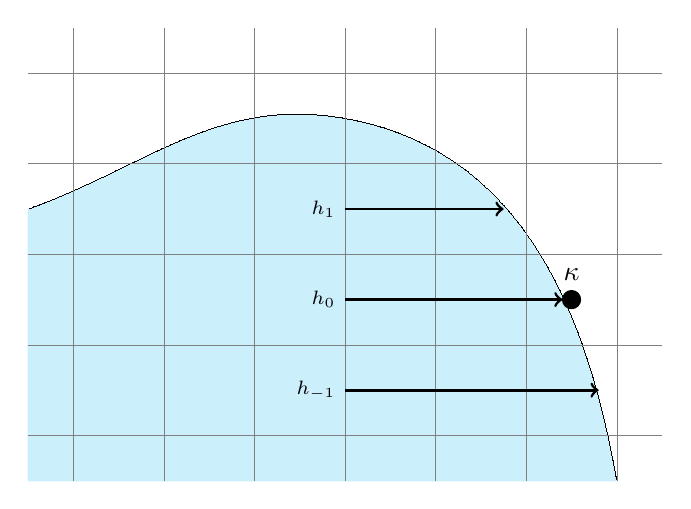
\begin{tikzpicture}[scale=1.15]
	% Mesh
	\draw [step=1.0, help lines] (0.5,0.5) grid (7.5,5.5);
	% Liquid
	\draw [line width=0,fill=cyan!20] (0.5,3.5) to[out=20,in=170] (4,4.5) to[out=-10,in=100] (7.0,0.5);
	\draw [cyan!20,fill=cyan!20] (0.5,3.5) -- (7.0,0.5) -- (0.5,0.5) -- cycle;
	\draw [step=1.0, help lines] (0.5,0.5) grid (7.5,5.5);
	% kappa 1
	\draw [fill] (6.5,2.5) circle [radius=0.1];
	\node [above ] at (6.5,2.6) {$\kappa$};
	\draw [arrows=->,line width=1.0] (4.0,1.5) -- (6.8,1.5);\node [left] at (4.0,1.5) {\scriptsize $h_{-1}$};
	\draw [arrows=->,line width=1.0] (4.0,2.5) -- (6.4,2.5);\node [left] at (4.0,2.5) {\scriptsize $h_{0}$};
	\draw [arrows=->,line width=1.0] (4.0,3.5) -- (5.75,3.5);\node [left] at (4.0,3.5) {\scriptsize $h_{1}$};
	\end{tikzpicture}
	\caption{Height function with a three cell stencil using widths.} 
	\label{fig:widths}
\end{figure}

Height functions remain a prevalent method for estimating curvature because of their relative ease of implementation and their second order convergence. However, several adjustments to the standard model have been proposed. Adjustments include changing the stencil size over which the heights are computed~\cite{Sussman2007, Sussman2003}, separating the columns from the computational mesh~\cite{Owkes2015}, combining heights and widths~\cite{Popinet2009}, and applying the approach to level sets~\cite{Owkes2013}.